\documentclass[aspectratio=169]{beamer}

\usepackage{amsmath,amssymb}
\usepackage{graphicx}
\usepackage{tikz}
\usepackage{listings}
\usepackage[edges]{forest}
\usetikzlibrary{positioning,calc,arrows.meta,fit,shapes.multipart}

% =========================
% Colors
% =========================
\definecolor{PKUDarkPurple}{RGB}{63,63,191}
\definecolor{PKULightPurple}{RGB}{170,170,225}
\definecolor{PKUGrayBg}{RGB}{255,255,255}
\definecolor{PKUTextBlue}{RGB}{45,45,190}
\definecolor{CodeGray}{RGB}{245,245,245}
\definecolor{dkgreen}{rgb}{0,0.5,0}
\definecolor{gray}{rgb}{0.4,0.4,0.4}
\definecolor{mauve}{rgb}{0.58,0,0.82}

% =========================
% Global style
% =========================
\setbeamercolor{background canvas}{bg=PKUGrayBg}
\setbeamercolor{normal text}{fg=black,bg=PKUGrayBg}
\setbeamercolor{frametitle}{fg=PKUTextBlue,bg=PKUGrayBg}

\setbeamerfont{normal text}{size=\fontsize{15pt}{18pt}\selectfont}
\setbeamerfont{frametitle}{size=\fontsize{15pt}{19pt}\selectfont,series=\bfseries}
\setbeamerfont{itemize/enumerate body}{size=\fontsize{12pt}{15pt}\selectfont}
\setbeamerfont{itemize/enumerate subbody}{size=\fontsize{11pt}{14pt}\selectfont}
\setbeamerfont{footline}{size=\fontsize{10pt}{12pt}\selectfont}

\setbeamercolor{itemize item}{fg=PKUDarkPurple}
\setbeamertemplate{navigation symbols}{}
\setbeamertemplate{items}[ball]
\setbeamertemplate{headline}{}
\setbeamertemplate{footline}{}

% =========================
% Code style
% =========================
\lstset{
  basicstyle=\ttfamily\footnotesize,
  backgroundcolor=\color{CodeGray},
  keywordstyle=\color{blue},
  commentstyle=\color{dkgreen},
  stringstyle=\color{mauve},
  showstringspaces=false,
  breaklines=true,
  frame=single,
  columns=fullflexible
}

% =========================
% Custom headline and footline
% =========================
\newcommand{\makecustomheadline}{
\begin{tikzpicture}[remember picture,overlay]
    \fill[PKUDarkPurple]
        (current page.north west)
        rectangle
        ([xshift=.50\paperwidth,yshift=-0.35cm]current page.north west);

    \fill[PKULightPurple]
        ([xshift=.50\paperwidth]current page.north west)
        rectangle
        ([xshift=\paperwidth,yshift=-0.35cm]current page.north west);
\end{tikzpicture}
}

\newcommand{\makecustomfootline}{
\begin{tikzpicture}[remember picture,overlay]
    \fill[PKUDarkPurple]
        (current page.south west)
        rectangle
        ([xshift=.33\paperwidth,yshift=0.42cm]current page.south west);

    \fill[PKULightPurple]
        ([xshift=.33\paperwidth]current page.south west)
        rectangle
        ([xshift=.67\paperwidth,yshift=0.42cm]current page.south west);

    \fill[PKULightPurple]
        ([xshift=.67\paperwidth]current page.south west)
        rectangle
        ([xshift=\paperwidth,yshift=0.42cm]current page.south west);

    \node[anchor=center, text=white, font=\small]
        at ([xshift=.165\paperwidth,yshift=0.21cm]current page.south west)
        {\textrm{huangxun@pku.edu.cn}};

    \node[anchor=center, text=white, font=\small]
        at ([xshift=.50\paperwidth,yshift=0.21cm]current page.south west)
        {AI Enabled Control Engineering};

    \node[anchor=center, text=black, font=\small]
        at ([xshift=.83\paperwidth,yshift=0.21cm]current page.south west)
        {2026 Summer};

    \node[anchor=center, text=black, font=\small]
        at ([xshift=.965\paperwidth,yshift=0.21cm]current page.south west)
        {\insertframenumber/\inserttotalframenumber};
\end{tikzpicture}
}

\addtobeamertemplate{background}{\makecustomheadline\makecustomfootline}{}

\title{\textcolor{PKUTextBlue}{AI Enabled Control Engineering}}
\author{\textcolor{blue}{Professor Xun Huang}}
\institute{
Aeronautics and Astronautics\\
College of Engineering\\
Peking University\\[0.25cm]
huangxun@pku.edu.cn\\
https://xunger99.github.io/xunger/
}
\date{}

\setbeamertemplate{title page}{
    \vspace{1.0cm}
    \begin{center}
        {\fontsize{18}{22}\selectfont\bfseries \inserttitle\par}
        \vspace{0.3cm}
        {\fontsize{15}{18}\selectfont Lecture 10: Simulation Training of DQN, PPO, and TD3 for the Rotary Inverted Pendulum\par}
          \vspace{0.3cm}
        {\fontsize{15}{18}\selectfont \insertauthor\par}
        \vspace{0.15cm}
        {\fontsize{11}{13}\selectfont TA: Zhixiang Ju \quad Haozhe Wang\par}
        \vspace{0.4cm}
        {\fontsize{8}{11}\selectfont \insertinstitute\par}
    \end{center}
}

\begin{document}

% ---------------------------------
\begin{frame}
\titlepage
\end{frame}

% ---------------------------------
% ---------------------------------
\begin{frame}{Common classification of reinforcement learning algorithms}

\begin{center}
\resizebox{0.95\textwidth}{!}{
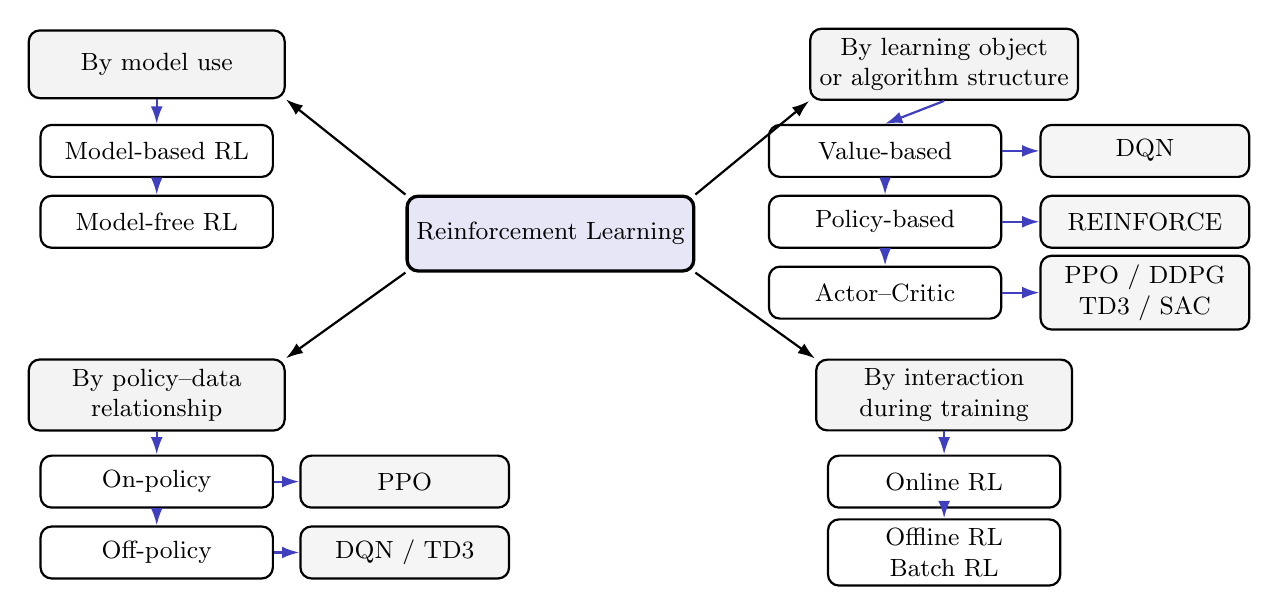
\begin{tikzpicture}[
    font=\small,
    >={Latex[length=2.3mm,width=1.6mm]},
    main/.style={
        draw,
        rounded corners=4pt,
        very thick,
        align=center,
        minimum width=3.4cm,
        minimum height=0.95cm,
        fill=PKULightPurple!30
    },
    titlebox/.style={
        draw,
        rounded corners=4pt,
        thick,
        align=center,
        minimum width=3.25cm,
        minimum height=0.86cm,
        fill=gray!8
    },
    itembox/.style={
        draw,
        rounded corners=4pt,
        thick,
        align=center,
        minimum width=2.95cm,
        minimum height=0.66cm,
        fill=white
    },
    algobox/.style={
        draw,
        rounded corners=4pt,
        thick,
        align=center,
        minimum width=2.65cm,
        minimum height=0.66cm,
        fill=CodeGray
    },
    arrow/.style={
        -{Latex[length=2.2mm,width=1.5mm]},
        thick,
        draw=black
    },
    bluearrow/.style={
        -{Latex[length=2.2mm,width=1.5mm]},
        thick,
        draw=PKUDarkPurple
    }
]

% center
\node[main] (rl) at (0,0) {Reinforcement Learning};

% =========================
% upper-left: model use
% =========================
\node[titlebox] (modeltitle) at (-5.0,2.15) {By model use};

\node[itembox] (mb) at (-5.0,1.05) {Model-based RL};
\node[itembox] (mf) at (-5.0,0.15) {Model-free RL};

\draw[arrow] (rl.north west) -- (modeltitle.south east);
\draw[bluearrow] (modeltitle.south) -- (mb.north);
\draw[bluearrow] (mb.south) -- (mf.north);

% =========================
% upper-right: learning object
% =========================
\node[titlebox] (objecttitle) at (5.0,2.15) {By learning object\\or algorithm structure};

\node[itembox] (value) at (4.25,1.05) {Value-based};
\node[algobox] (dqn) at (7.55,1.05) {DQN};

\node[itembox] (policy) at (4.25,0.15) {Policy-based};
\node[algobox] (reinforce) at (7.55,0.15) {REINFORCE};

\node[itembox] (ac) at (4.25,-0.75) {Actor--Critic};
\node[algobox] (acalg) at (7.55,-0.75) {PPO / DDPG\\TD3 / SAC};

\draw[arrow] (rl.north east) -- (objecttitle.south west);
\draw[bluearrow] (objecttitle.south) -- (value.north);
\draw[bluearrow] (value.south) -- (policy.north);
\draw[bluearrow] (policy.south) -- (ac.north);

\draw[bluearrow] (value.east) -- (dqn.west);
\draw[bluearrow] (policy.east) -- (reinforce.west);
\draw[bluearrow] (ac.east) -- (acalg.west);

% =========================
% lower-left: policy/data relation
% =========================
\node[titlebox] (datatitle) at (-5.0,-2.05) {By policy--data\\relationship};

\node[itembox] (on) at (-5.0,-3.15) {On-policy};
\node[algobox] (ppo) at (-1.85,-3.15) {PPO};

\node[itembox] (off) at (-5.0,-4.05) {Off-policy};
\node[algobox] (offalg) at (-1.85,-4.05) {DQN / TD3};

\draw[arrow] (rl.south west) -- (datatitle.north east);
\draw[bluearrow] (datatitle.south) -- (on.north);
\draw[bluearrow] (on.south) -- (off.north);

\draw[bluearrow] (on.east) -- (ppo.west);
\draw[bluearrow] (off.east) -- (offalg.west);

% =========================
% lower-right: online/offline
% =========================
\node[titlebox] (interacttitle) at (5.0,-2.05) {By interaction\\during training};

\node[itembox] (online) at (5.0,-3.15) {Online RL};
\node[itembox] (offline) at (5.0,-4.05) {Offline RL\\Batch RL};

\draw[arrow] (rl.south east) -- (interacttitle.north west);
\draw[bluearrow] (interacttitle.south) -- (online.north);
\draw[bluearrow] (online.south) -- (offline.north);

\end{tikzpicture}
}
\end{center}

\end{frame}
% ---------------------------------

% ---------------------------------
\begin{frame}{Why simulation training first?}

\begin{itemize}
    \item Real RIP training may be unsafe and time-consuming.
    \vspace{0.2cm}

    \item Simulation allows many episodes, random initial states, and fast hyperparameter search.
    \vspace{0.2cm}

    \item In simulation, time is virtual: training update does not violate a real \(5\,\mathrm{ms}\) control period.
    \vspace{0.2cm}

    \item A good simulation policy can be used for pretraining, algorithm selection, and deployment testing.
\end{itemize}

\vspace{0.2cm}

\begin{alertblock}{But simulation is not the real system}
\small
Model mismatch, motor dead zone, friction, sensor noise, and communication delay may still degrade real-system performance.
\end{alertblock}

\end{frame}


% ---------------------------------
\begin{frame}{Reinforcement learning problem}

\begin{center}
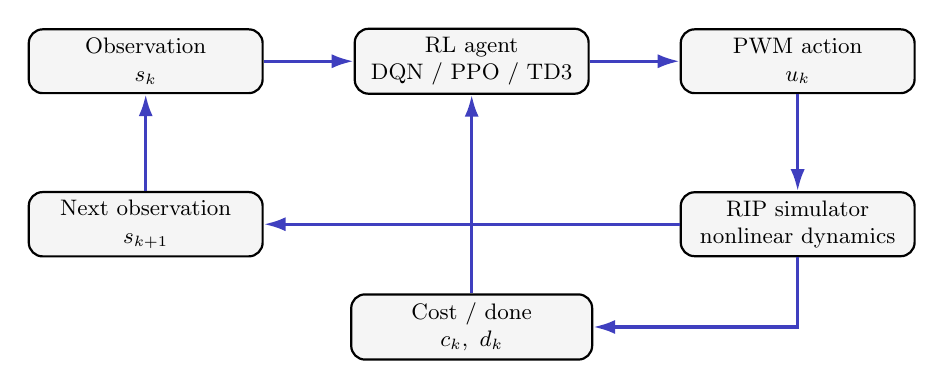
\begin{tikzpicture}[
    scale=0.90,
    transform shape,
    font=\small,
    >={Latex[length=2.8mm,width=1.8mm]},
    block/.style={
        draw,
        rounded corners=5pt,
        thick,
        align=center,
        minimum width=3.3cm,
        minimum height=0.9cm,
        fill=CodeGray
    },
    arrow/.style={
        ->,
        very thick,
        draw=PKUDarkPurple
    }
]

\node[block] (obs) at (-4.6,1.3) {Observation\\$s_k$};
\node[block] (agent) at (0,1.3) {RL agent\\DQN / PPO / TD3};
\node[block] (action) at (4.6,1.3) {PWM action\\$u_k$};

\node[block] (env) at (4.6,-1.0) {RIP simulator\\nonlinear dynamics};
\node[block] (nextobs) at (-4.6,-1.0) {Next observation\\$s_{k+1}$};

\node[block, minimum width=3.4cm] (reward) at (0,-2.45) {Cost / done\\$c_k,\ d_k$};

\draw[arrow] (obs.east) -- (agent.west);
\draw[arrow] (agent.east) -- (action.west);
\draw[arrow] (action.south) -- (env.north);

\draw[arrow] (env.west) -- (nextobs.east);
\draw[arrow] (nextobs.north) -- (obs.south);

\draw[arrow] (env.south) |- (reward.east);
\draw[arrow] (reward.north) -- (agent.south);

\end{tikzpicture}
\end{center}



\begin{block}{One environment step}
\small
At step \(k\), the agent observes \(s_k\), outputs action \(u_k\), and the simulator returns
\[
s_{k+1},\qquad c_k,\qquad d_k .
\]

\end{block}

\end{frame}


% ---------------------------------
\begin{frame}{Q-learning idea: a table of state--action costs}

For discrete states and discrete actions, we may store one value for every pair:
\[
Q(s,a).
\]

\vspace{0.15cm}

\begin{center}
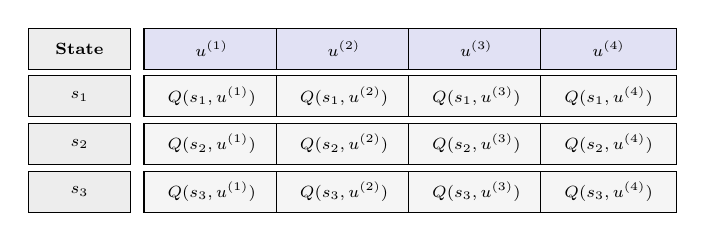
\begin{tikzpicture}[
    scale=0.84,
    transform shape,
    font=\scriptsize,
    cell/.style={
        draw,
        minimum width=2.05cm,
        minimum height=0.62cm,
        align=center,
        fill=CodeGray
    },
    head/.style={
        draw,
        minimum width=2.05cm,
        minimum height=0.62cm,
        align=center,
        fill=PKULightPurple!35,
        font=\scriptsize\bfseries
    },
    state/.style={
        draw,
        minimum width=1.55cm,
        minimum height=0.62cm,
        align=center,
        fill=gray!12,
        font=\scriptsize\bfseries
    }
]

\node[state] at (0,0) {State};
\node[head] at (2.0,0) {$u^{(1)}$};
\node[head] at (4.0,0) {$u^{(2)}$};
\node[head] at (6.0,0) {$u^{(3)}$};
\node[head] at (8.0,0) {$u^{(4)}$};

\node[state] at (0,-0.72) {$s_1$};
\node[cell] at (2.0,-0.72) {$Q(s_1,u^{(1)})$};
\node[cell] at (4.0,-0.72) {$Q(s_1,u^{(2)})$};
\node[cell] at (6.0,-0.72) {$Q(s_1,u^{(3)})$};
\node[cell] at (8.0,-0.72) {$Q(s_1,u^{(4)})$};

\node[state] at (0,-1.44) {$s_2$};
\node[cell] at (2.0,-1.44) {$Q(s_2,u^{(1)})$};
\node[cell] at (4.0,-1.44) {$Q(s_2,u^{(2)})$};
\node[cell] at (6.0,-1.44) {$Q(s_2,u^{(3)})$};
\node[cell] at (8.0,-1.44) {$Q(s_2,u^{(4)})$};

\node[state] at (0,-2.16) {$s_3$};
\node[cell] at (2.0,-2.16) {$Q(s_3,u^{(1)})$};
\node[cell] at (4.0,-2.16) {$Q(s_3,u^{(2)})$};
\node[cell] at (6.0,-2.16) {$Q(s_3,u^{(3)})$};
\node[cell] at (8.0,-2.16) {$Q(s_3,u^{(4)})$};

\end{tikzpicture}
\end{center}

\vspace{0.1cm}

\begin{block}{Meaning}
\small
\(Q(s,a)\) means: after taking action \(a\) at state \(s\), how large the long-term cost will be if we act optimally afterwards.
For cost minimization,
\[
a^*(s)=\arg\min_a Q(s,a).
\]
\end{block}

\end{frame}


% ---------------------------------
\begin{frame}{Q-learning update from one transition}

At step \(k\), the environment gives one transition sample:
\[
(s_k,a_k,c_k,s_{k+1},d_k).
\]



The Bellman target is
\[
y_k
=
c_k
+
\Gamma(1-d_k)
\min_{a'}Q(s_{k+1},a').
\]



Q-learning updates only the visited table entry:
\[
Q(s_k,a_k)
\leftarrow
Q(s_k,a_k)
+
\eta
\left[
y_k-Q(s_k,a_k)
\right].
\]



\begin{block}{TD error}
\small
\[
\delta_k=y_k-Q(s_k,a_k).
\]
\end{block}

\end{frame}


% ---------------------------------
\begin{frame}{Why tabular Q-learning is not enough}

Tabular Q-learning is intuitive, but it requires a finite table.

\vspace{0.2cm}

For the rotary inverted pendulum, the physical state is continuous:
\[
x=
\begin{bmatrix}
\theta & \dot\theta & \alpha & \dot\alpha
\end{bmatrix}^{\top}.
\]

\vspace{0.2cm}

Even if the action set is finite, the number of possible states is still extremely large.

\vspace{0.2cm}

\begin{alertblock}{Problem}
\small
We cannot store one table entry for every possible state--action pair.
Therefore, we need a function approximator.
\end{alertblock}

\vspace{0.15cm}

DQN replaces the Q-table by a neural network:
\[
Q_\theta(s,a)\approx Q^*(s,a).
\]

\end{frame}


% ---------------------------------
\begin{frame}{DQN: replacing the Q-table by a neural network}

\begin{center}
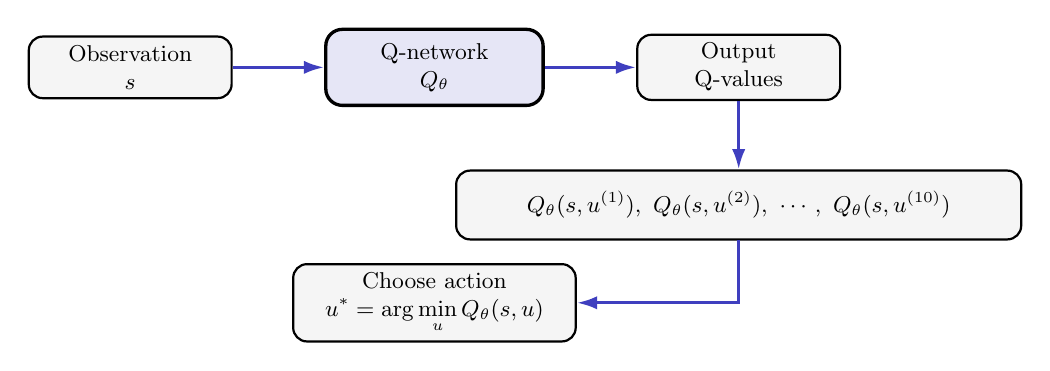
\begin{tikzpicture}[
    scale=0.92,
    transform shape,
    font=\small,
    >={Latex[length=2.6mm,width=1.7mm]},
    block/.style={
        draw,
        rounded corners=5pt,
        thick,
        align=center,
        minimum width=2.8cm,
        minimum height=0.85cm,
        fill=CodeGray
    },
    net/.style={
        draw,
        rounded corners=6pt,
        very thick,
        align=center,
        minimum width=3.0cm,
        minimum height=1.05cm,
        fill=PKULightPurple!30
    },
    arrow/.style={
        ->,
        very thick,
        draw=PKUDarkPurple
    }
]

\node[block] (snode) at (-4.2,0.9) {Observation\\$s$};
\node[net] (qnet) at (0,0.9) {Q-network\\$Q_\theta$};
\node[block] (qout) at (4.2,0.9) {Output\\Q-values};

\draw[arrow] (snode.east) -- (qnet.west);
\draw[arrow] (qnet.east) -- (qout.west);

\node[
    block,
    minimum width=7.8cm,
    minimum height=0.95cm
] (actions) at (4.2,-1.0)
{$Q_\theta(s,u^{(1)}),\ Q_\theta(s,u^{(2)}),\ \cdots,\ Q_\theta(s,u^{(10)})$};

\draw[arrow] (qout.south) -- (actions.north);

\node[block, minimum width=3.9cm] (choose) at (0,-2.35)
{Choose action\\$\displaystyle u^*=\arg\min_u Q_\theta(s,u)$};

\draw[arrow] (actions.south) |- (choose.east);

\end{tikzpicture}
\end{center}

\vspace{0.1cm}

\begin{block}{For DQN in this class}
\small
The network receives the observation \(s\) and outputs one Q-value for each discrete action.
The action with the smallest predicted cost is selected during exploitation.
\end{block}

\end{frame}


% ---------------------------------
\begin{frame}{DQN key component 1: experience replay}

During interaction, store transitions into a replay buffer:
\[
\mathcal D
=
\left\{
(s_k,a_k,c_k,s_{k+1},d_k)
\right\}.
\]

\vspace{0.15cm}

\begin{center}
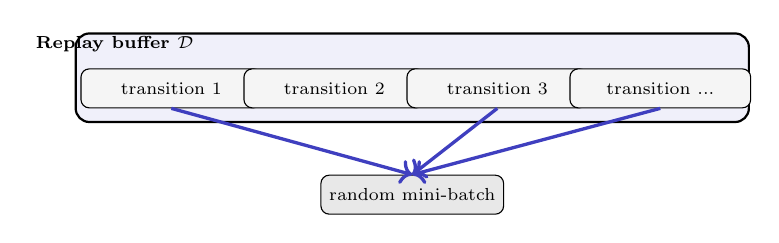
\begin{tikzpicture}[
    scale=0.90,
    transform shape,
    font=\scriptsize,
    trans/.style={
        draw,
        rounded corners=3pt,
        minimum width=2.55cm,
        minimum height=0.55cm,
        align=center,
        fill=CodeGray
    },
    buf/.style={
        draw,
        rounded corners=5pt,
        thick,
        minimum width=9.5cm,
        minimum height=1.25cm,
        fill=PKULightPurple!18
    },
    arrow/.style={
        ->,
        very thick,
        draw=PKUDarkPurple
    }
]

\node[buf] (buffer) at (0,0) {};
\node at (-4.2,0.48) {\textbf{Replay buffer \(\mathcal D\)}};

\node[trans] (t1) at (-3.4,-0.15) {transition 1};
\node[trans] (t2) at (-1.1,-0.15) {transition 2};
\node[trans] (t3) at (1.2,-0.15) {transition 3};
\node[trans] (t4) at (3.5,-0.15) {transition ...};

\node[trans, fill=gray!15] (sample) at (0,-1.65) {random mini-batch};

\draw[arrow] (t1.south) -- (sample.north);
\draw[arrow] (t3.south) -- (sample.north);
\draw[arrow] (t4.south) -- (sample.north);

\end{tikzpicture}
\end{center}

\vspace{0.1cm}

\begin{itemize}
    \item Random mini-batches break temporal correlation.
    \item Old swing-up and balancing experiences can be reused many times.
\end{itemize}

\end{frame}


% ---------------------------------
\begin{frame}{DQN key component 2: online network and target network}

DQN uses two networks:

\vspace{0.15cm}

\begin{center}
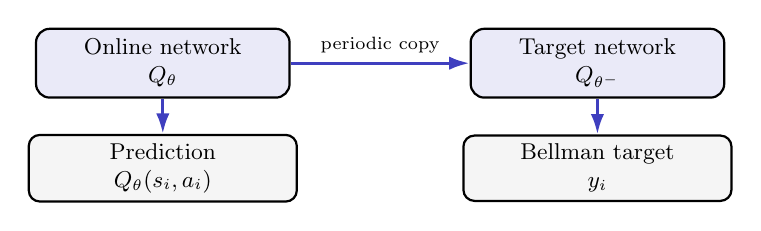
\begin{tikzpicture}[
    scale=0.92,
    transform shape,
    font=\small,
    >={Latex[length=2.6mm,width=1.7mm]},
    net/.style={
        draw,
        rounded corners=5pt,
        thick,
        align=center,
        minimum width=3.5cm,
        minimum height=0.95cm,
        fill=PKULightPurple!25
    },
    block/.style={
        draw,
        rounded corners=4pt,
        thick,
        align=center,
        minimum width=3.7cm,
        minimum height=0.85cm,
        fill=CodeGray
    },
    arrow/.style={
        ->,
        very thick,
        draw=PKUDarkPurple
    }
]

\node[net] (online) at (-3.0,1.0) {Online network\\$Q_\theta$};
\node[block] (pred) at (-3.0,-0.45) {Prediction\\$Q_\theta(s_i,a_i)$};

\node[net] (target) at (3.0,1.0) {Target network\\$Q_{\theta^-}$};
\node[block] (tar) at (3.0,-0.45) {Bellman target\\$y_i$};

\draw[arrow] (online.south) -- (pred.north);
\draw[arrow] (target.south) -- (tar.north);

\draw[arrow] (online.east) -- node[above] {\scriptsize periodic copy} (target.west);

\end{tikzpicture}
\end{center}

\vspace{0.15cm}

The target is computed by the delayed network:
\[
y_i=c_i+\Gamma(1-d_i)\min_{a'}Q_{\theta^-}(s'_i,a').
\]

\vspace{0.1cm}

\begin{block}{Effect}
\small
The target network makes the Bellman target more stable during training.
\end{block}

\end{frame}


% ---------------------------------
\begin{frame}{DQN key component 3: \(\epsilon\)-greedy exploration}

DQN selects actions by an \(\epsilon\)-greedy behavior policy:
\[
a_k=
\begin{cases}
\text{random action from }\mathcal U_d, & \text{with probability }\epsilon,\\
\arg\min_a Q_\theta(s_k,a), & \text{with probability }1-\epsilon.
\end{cases}
\]

\vspace{0.2cm}

\begin{itemize}
    \item Large \(\epsilon\): more random exploration at the beginning.
    \vspace{0.2cm}

    \item Small \(\epsilon\): more use of the learned Q-network.
    \vspace{0.2cm}

    \item In practice, \(\epsilon\) gradually decays during training.
\end{itemize}

\vspace{0.15cm}

\begin{block}{For RIP simulation}
\small
Exploration allows the agent to try different PWM actions and discover useful swing-up and balancing behaviors.
\end{block}

\end{frame}


% ---------------------------------
\begin{frame}{DQN loss function}

\small
Given a mini-batch
\[
\{(s_i,a_i,c_i,s'_i,d_i)\}_{i=1}^{B},
\]
construct the Bellman target
\[
y_i=c_i+\Gamma(1-d_i)\min_{a'}Q_{\theta^-}(s'_i,a').
\]

\vspace{-0.1cm}

The mini-batch loss is
\[
\mathcal L_B(\theta)=
\frac{1}{B}\sum_{i=1}^{B}
\frac12\left[y_i-Q_\theta(s_i,a_i)\right]^2.
\]

\vspace{-0.1cm}

Update the online network:
\[
\theta\leftarrow\theta-\eta\nabla_\theta \mathcal L_B(\theta).
\]

\vspace{-0.05cm}

\begin{block}{TD error}
\small
\[
\delta_i=y_i-Q_\theta(s_i,a_i).
\]
DQN trains the network by reducing this sample Bellman residual.
\end{block}

\end{frame}
% ---------------------------------
\begin{frame}{DQN training workflow: compact table view}

\scriptsize

\begin{columns}[T,totalwidth=\textwidth]

% ================= left column =================
\begin{column}{0.49\textwidth}

\begin{block}{Interaction and data collection}
\begin{tabular}{c|p{0.78\linewidth}}
\hline
\textbf{Step} & \textbf{Operation} \\
\hline
1 & Initialize \(Q_\theta\), \(Q_{\theta^-}\), replay buffer \(\mathcal D\), and RIP environment. \\
\hline
2 & Reset simulator and obtain initial observation \(s_0\). \\
\hline
3 & Select action by \(\epsilon\)-greedy policy. \\
\hline
4 & Map action index \(a_k\) to discrete PWM command \(u_k\). \\
\hline
5 & Run one nonlinear simulator step:
\[
(s_{k+1},c_k,d_k)=\texttt{env.step}(u_k).
\]
\\
\hline
6 & Store transition:
\[
\mathcal D\leftarrow
\mathcal D\cup(s_k,a_k,c_k,s_{k+1},d_k).
\]
\\
\hline
\end{tabular}
\end{block}

\end{column}

% ================= right column =================
\begin{column}{0.49\textwidth}

\begin{block}{Network training and saving}
\begin{tabular}{c|p{0.78\linewidth}}
\hline
\textbf{Step} & \textbf{Operation} \\
\hline
7 & After warm-up, sample a mini-batch from replay buffer \(\mathcal D\). \\
\hline
8 & Build Bellman target using the target network:
\[
y_i=c_i+\Gamma(1-d_i)\min_{a'}Q_{\theta^-}(s'_i,a').
\]
\\
\hline
9 & Minimize Bellman residual and update online network \(Q_\theta\). \\
\hline
10 & Periodically synchronize target network:
\[
\theta^-\leftarrow\theta.
\]
\\
\hline
11 & Evaluate current policy and save reward curves, logs, checkpoints, and config snapshots. \\
\hline
\end{tabular}
\end{block}

\end{column}

\end{columns}

\vspace{0.12cm}

\begin{alertblock}{Key point}
\small
The left column collects experience from the simulator; the right column uses replay-buffer samples to train the Q-network.
\end{alertblock}

\end{frame}

% ---------------------------------
\begin{frame}{DQN training workflow}

\begin{center}
\resizebox{0.94\textwidth}{!}{
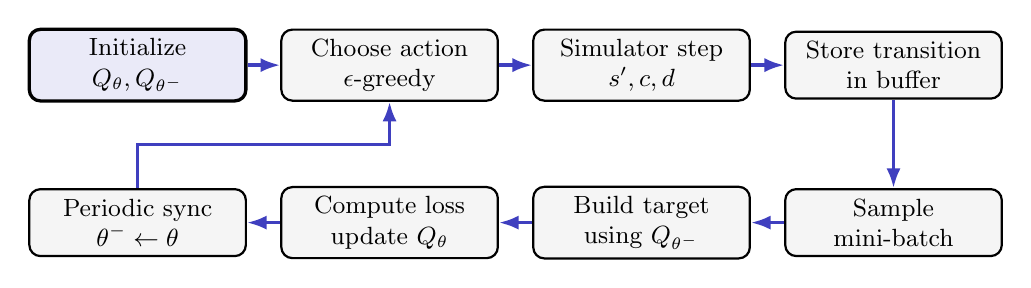
\begin{tikzpicture}[
    font=\small,
    >={Latex[length=2.5mm,width=1.8mm]},
    box/.style={
        draw,
        rounded corners=4pt,
        thick,
        align=center,
        minimum width=2.75cm,
        minimum height=0.85cm,
        fill=CodeGray
    },
    netbox/.style={
        draw,
        rounded corners=4pt,
        very thick,
        align=center,
        minimum width=2.75cm,
        minimum height=0.85cm,
        fill=PKULightPurple!25
    },
    arrow/.style={
        ->,
        very thick,
        draw=PKUDarkPurple
    }
]

\node[netbox] (init) at (0,0) {Initialize\\$Q_\theta,Q_{\theta^-}$};
\node[box] (act) at (3.2,0) {Choose action\\\(\epsilon\)-greedy};
\node[box] (step) at (6.4,0) {Simulator step\\$s',c,d$};
\node[box] (store) at (9.6,0) {Store transition\\in buffer};

\node[box] (sample) at (9.6,-2.0) {Sample\\mini-batch};
\node[box] (target) at (6.4,-2.0) {Build target\\using \(Q_{\theta^-}\)};
\node[box] (loss) at (3.2,-2.0) {Compute loss\\update \(Q_\theta\)};
\node[box] (sync) at (0,-2.0) {Periodic sync\\\(\theta^-\leftarrow\theta\)};

\draw[arrow] (init) -- (act);
\draw[arrow] (act) -- (step);
\draw[arrow] (step) -- (store);
\draw[arrow] (store) -- (sample);
\draw[arrow] (sample) -- (target);
\draw[arrow] (target) -- (loss);
\draw[arrow] (loss) -- (sync);
\draw[arrow] (sync.north) -- ++(0,0.55) -| (act.south);

\end{tikzpicture}
}
\end{center}

\vspace{0.1cm}

\begin{block}{Summary}
\small
DQN keeps the Q-learning Bellman update, but replaces the Q-table with a neural network trained from replay-buffer samples.
\end{block}

\end{frame}


% ---------------------------------
\begin{frame}{DQN for RIP: discrete PWM action space}
In the provided DQN setup, the action space is discrete:
\[
\mathcal U_d=
\{-150,-120,-90,-60,-30,30,60,90,120,150\}.
\]


The neural network outputs one Q value for each PWM action:
\[
Q_\theta(s,u^{(1)}),\ldots,Q_\theta(s,u^{(10)}).
\]


The selected control command is
\[
u_k=u^{(i^*)},
\qquad
 i^*=\arg\min_i Q_\theta(s_k,u^{(i)}).
\]

\begin{alertblock}{Cost-minimization convention}
\small
If the code uses reward maximization internally, the implementation may use \(\arg\max\). Always check whether the variable is reward or cost.
\end{alertblock}
\end{frame}

% ---------------------------------
\begin{frame}{Brief introduction to TD3}
TD3 is an off-policy Actor--Critic algorithm for continuous actions.

\vspace{0.2cm}
\begin{itemize}
    \item Actor network outputs a continuous action:
    \[
    u=\mu_\theta(s).
    \]

    \item Critic networks estimate action values:
    \[
    Q_{\phi_1}(s,u),\qquad Q_{\phi_2}(s,u).
    \]
 
    \item TD3 uses twin critics, target policy smoothing, and delayed actor updates.
\end{itemize}


TD3 can output continuous PWM values, but it may be more sensitive to model mismatch, actuator dead zones, and sim-to-real errors.

\end{frame}

% ---------------------------------
\begin{frame}{Brief introduction to PPO}
PPO is an on-policy Actor--Critic algorithm.


\begin{itemize}
    \item The actor outputs an action distribution.

    \item The critic estimates the state value $V(s)$.

    \item PPO updates the policy using recent trajectories collected by the current policy.
\end{itemize}


The clipped objective uses the probability ratio
\[
r_t(\theta)=\frac{\pi_\theta(a_t|s_t)}{\pi_{\theta_{old}}(a_t|s_t)}
\]
and restricts overly large policy updates.


PPO can be stable in simulation, but on-policy training is usually less sample-efficient than replay-buffer based methods.

\end{frame}

% ---------------------------------
\begin{frame}{DQN, PPO, and TD3 at a glance}
\begin{center}
\begin{tabular}{c|c|c|c}
\hline
Algorithm & Main type & Action space & Data usage \\
\hline
DQN & value-based & discrete & off-policy replay \\
PPO & Actor--Critic & discrete/continuous & on-policy trajectories \\
TD3 & Actor--Critic & continuous & off-policy replay \\
\hline
\end{tabular}
\end{center}

\vspace{0.35cm}
\begin{itemize}
    \item DQN: simplest connection to Q-learning and Bellman targets.
    \vspace{0.18cm}
    \item PPO: stable policy update through clipped policy optimization.
    \vspace{0.18cm}
    \item TD3: continuous control with twin critics and delayed policy updates.
\end{itemize}
\end{frame}

% ---------------------------------
\begin{frame}{Part II: RIP simulation training environment}
\begin{itemize}
    \item The RIP simulator is written as a Gymnasium-style environment.
    \vspace{0.22cm}
    \item The environment implements nonlinear dynamics, numerical integration, reward, termination, and logging.
    \vspace{0.22cm}
    \item The training script calls Stable-Baselines3 style algorithms.
    \vspace{0.22cm}
    \item DQN, PPO, and TD3 can share the same physical environment interface.
\end{itemize}


\end{frame}

% ---------------------------------
% ---------------------------------
% ---------------------------------
\begin{frame}{Project file tree}

\begin{center}
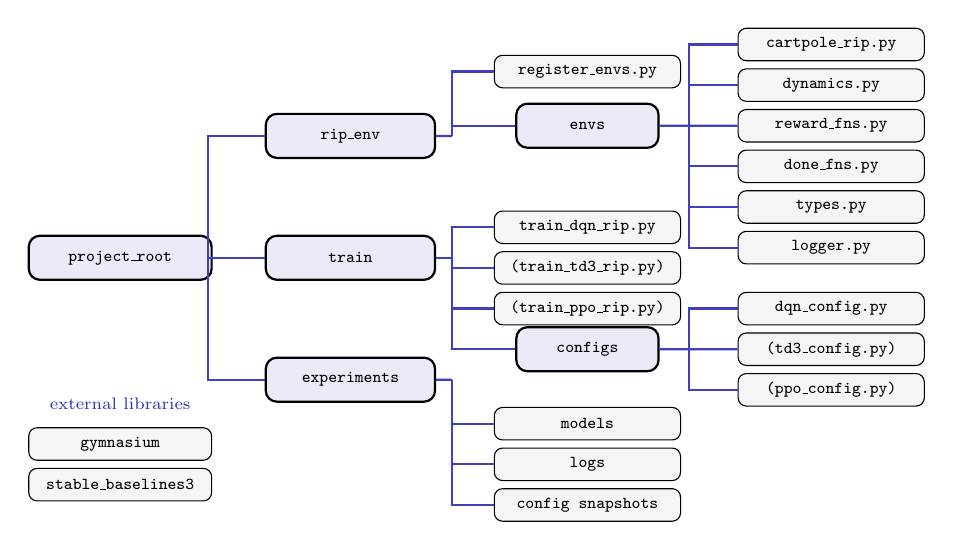
\begin{tikzpicture}[
    scale=0.86,
    transform shape,
    font=\ttfamily\scriptsize,
    >={Latex[length=2.2mm,width=1.5mm]},
    folder/.style={
        draw,
        thick,
        rounded corners=4pt,
        minimum width=2.5cm,
        minimum height=0.65cm,
        align=center,
        fill=PKULightPurple!25
    },
    file/.style={
        draw,
        rounded corners=3pt,
        minimum width=2.75cm,
        minimum height=0.48cm,
        align=center,
        fill=CodeGray
    },
    arrow/.style={
        -,
        thick,
        draw=PKUDarkPurple
    }
]

% root
\node[folder, minimum width=2.7cm] (root) at (-5.9,0) {project\_root};

% middle folders
\node[folder] (ripenv) at (-2.5,1.8) {rip\_env};
\node[folder] (train)  at (-2.5,0.0) {train};
\node[folder] (exp)    at (-2.5,-1.8) {experiments};

\draw[arrow] (root.east) -- (-4.6,0);
\draw[arrow] (-4.6,0) |- (ripenv.west);
\draw[arrow] (-4.6,0) -- (train.west);
\draw[arrow] (-4.6,0) |- (exp.west);

% rip_env details
\node[file] (reg) at (1.0,2.75) {register\_envs.py};
\node[folder, minimum width=2.1cm] (envs) at (1.0,1.95) {envs};

\draw[arrow] (ripenv.east) -- (-1.0,1.8);
\draw[arrow] (-1.0,1.8) |- (reg.west);
\draw[arrow] (-1.0,1.8) |- (envs.west);

\node[file] (cart) at (4.6,3.15) {cartpole\_rip.py};
\node[file] (dyn)  at (4.6,2.55) {dynamics.py};
\node[file] (rew)  at (4.6,1.95) {reward\_fns.py};
\node[file] (done) at (4.6,1.35) {done\_fns.py};
\node[file] (types) at (4.6,0.75) {types.py};
\node[file] (log) at (4.6,0.15) {logger.py};

\draw[arrow] (envs.east) -- (2.5,1.95);
\draw[arrow] (2.5,1.95) |- (cart.west);
\draw[arrow] (2.5,1.95) |- (dyn.west);
\draw[arrow] (2.5,1.95) -- (rew.west);
\draw[arrow] (2.5,1.95) |- (done.west);
\draw[arrow] (2.5,1.95) |- (types.west);
\draw[arrow] (2.5,1.95) |- (log.west);

% train details
\node[file] (dqn) at (1.0,0.45) {train\_dqn\_rip.py};
\node[file] (td3) at (1.0,-0.15) {(train\_td3\_rip.py)};
\node[file] (ppo) at (1.0,-0.75) {(train\_ppo\_rip.py)};
\node[folder, minimum width=2.1cm] (configs) at (1.0,-1.35) {configs};

\draw[arrow] (train.east) -- (-1.0,0);
\draw[arrow] (-1.0,0) |- (dqn.west);
\draw[arrow] (-1.0,0) |- (td3.west);
\draw[arrow] (-1.0,0) |- (ppo.west);
\draw[arrow] (-1.0,0) |- (configs.west);

\node[file] (dqnconf) at (4.6,-0.75) {dqn\_config.py};
\node[file] (td3conf) at (4.6,-1.35) {(td3\_config.py)};
\node[file] (ppoconf) at (4.6,-1.95) {(ppo\_config.py)};

\draw[arrow] (configs.east) -- (2.5,-1.35);
\draw[arrow] (2.5,-1.35) |- (dqnconf.west);
\draw[arrow] (2.5,-1.35) -- (td3conf.west);
\draw[arrow] (2.5,-1.35) |- (ppoconf.west);

% experiment outputs
\node[file] (models) at (1.0,-2.45) {models};
\node[file] (logs) at (1.0,-3.05) {logs};
\node[file] (snap) at (1.0,-3.65) {config snapshots};

\draw[arrow] (exp.east) -- (-1.0,-1.8);
\draw[arrow] (-1.0,-1.8) |- (models.west);
\draw[arrow] (-1.0,-1.8) |- (logs.west);
\draw[arrow] (-1.0,-1.8) |- (snap.west);

% external libs
\node[file, minimum width=2.7cm] (gym) at (-5.9,-2.75) {gymnasium};
\node[file, minimum width=2.7cm] (sb3) at (-5.9,-3.35) {stable\_baselines3};

\node[align=center, font=\scriptsize, text=PKUTextBlue] at (-5.9,-2.15) {external libraries};

\end{tikzpicture}
\end{center}

\vspace{-0.05cm}


\end{frame}

% ---------------------------------
\begin{frame}{Environment interface}
The environment follows the standard reinforcement learning interface:
\[
s_0=\texttt{env.reset()}.
\]

At each step:
\[
s_{k+1},r_k,d_k,\texttt{info}=\texttt{env.step}(a_k).
\]

\vspace{0.2cm}
Inside one environment step:
\begin{itemize}
    \item convert the selected action to PWM;
    \vspace{0.15cm}
    \item integrate the nonlinear RIP dynamics for one sampling interval;
    \vspace{0.15cm}
    \item compute observation, reward, and termination flag;
    \vspace{0.15cm}
    \item optionally write logs.
\end{itemize}
\end{frame}

% ---------------------------------
\begin{frame}{Important environment parameters}
\begin{center}
\begin{tabular}{c|c}
\hline
Item & Typical setting in the provided config \\
\hline
Sampling period & $\Delta t=0.005\,\mathrm{s}$ \\
Maximum episode length & 2000 steps \\
DQN action space size & 10 discrete PWM actions \\
DQN action values & student-defined discrete PWM set \\
Default velocity estimate & low-pass-filtered angle difference \\


\hline
\end{tabular}
\end{center}



\begin{block}{Action-space tuning}
\small
For DQN, the action space is limited to 10 discrete PWM actions.
Students may choose their own discrete action values, such as small, medium, or aggressive PWM levels.
\end{block}



\begin{alertblock}{Velocity estimation}
\small
The provided code uses low-pass-filtered angle differences by default.
Students may replace it with the observer designed in Lecture 9, but the report must clearly state which velocity-estimation method is used.
\end{alertblock}

\end{frame}
% ---------------------------------
\begin{frame}{DQN hyperparameters in the provided config}
\begin{center}
\begin{tabular}{c|c}
\hline
Parameter & Current value in provided config \\
\hline
\texttt{total\_timesteps} & $5.0\times 10^6$ \\
\texttt{learning\_rate} & $1.0\times 10^{-6}$ \\
\texttt{buffer\_size} & 30000 \\
\texttt{learning\_starts} & 2000 \\
\texttt{batch\_size} & 512 \\
\texttt{gamma} & 0.95 \\
\texttt{target\_update\_interval} & 2000 \\
\texttt{net\_arch} & (64, 64) \\
\texttt{exploration\_initial\_eps} & 1.0 \\
\texttt{exploration\_final\_eps} & 0.001 \\
\texttt{exploration\_decay} & 400000 \\
\hline
\end{tabular}
\end{center}
\end{frame}

% ---------------------------------
\begin{frame}[fragile]{How to run DQN training}
\begin{enumerate}
    \item Open a terminal in the project root.
    \vspace{0.18cm}
    \item Make sure the Python environment has required packages installed.
    \vspace{0.18cm}
    \item Run the DQN training entry point:
\end{enumerate}

\begin{lstlisting}[basicstyle=\ttfamily\small]
python train/train_dqn_rip.py
\end{lstlisting}

\vspace{0.15cm}
The script will:
\begin{itemize}
    \item register the custom RIP environment;
    \item build the environment, reward function, and termination function;
    \item create the DQN model;
    \item run training and periodically save checkpoints;
    \item save the final model and evaluation logs.
\end{itemize}
\end{frame}

% ---------------------------------
\begin{frame}{Training output files}
After running the training script, check the experiment folder:
\[
\texttt{experiments/dqn\_rip\_YYYYMMDD\_HHMMSS/}
\]

\vspace{0.15cm}
Typical contents:
\begin{itemize}
    \item \texttt{run\_config.json}: training hyperparameter snapshot;
    \vspace{0.15cm}
    \item \texttt{env\_config\_snapshot.json}: environment configuration snapshot;
    \vspace{0.15cm}
    \item \texttt{models/}: checkpoint and final model files;
    \vspace{0.15cm}
    \item \texttt{best\_model/}: best evaluation model;
    \vspace{0.15cm}
    \item \texttt{eval\_logs/}: evaluation statistics;
    \vspace{0.15cm}
    \item \texttt{env\_logs/}: episode or step logs if enabled.
\end{itemize}
\end{frame}

% ---------------------------------
\begin{frame}{What students should tune}
\begin{itemize}
    \item Learning rate: too large may be unstable; too small may learn slowly.
    \vspace{0.2cm}
    \item Exploration schedule: controls early exploration and later exploitation.
    \vspace{0.2cm}
    \item Reward weights: decide whether the policy prioritizes swing-up, balance, or small PWM.
    \vspace{0.2cm}
    \item Action set: coarse actions are robust but less smooth; fine actions require more learning.
    \vspace{0.2cm}
    \item Termination conditions: affect safety and the learning signal.
    \vspace{0.2cm}
    \item Network size and batch size: affect training speed and stability.
\end{itemize}
\end{frame}

% ---------------------------------
\begin{frame}[fragile]{Example: where to modify hyperparameters}
\begin{lstlisting}[basicstyle=\ttfamily\tiny]
# train/configs/dqn_config.py
@dataclass
class DQNRunConfig:
    total_timesteps: int = 5_000_000
    learning_rate: float = 1e-6
    buffer_size: int = 30_000
    learning_starts: int = 2_000
    batch_size: int = 512
    gamma: float = 0.95
    target_update_interval: int = 2000
    exploration_initial_eps: float = 1.0
    exploration_final_eps: float = 0.001
    exploration_decay: float = 400000.0
    net_arch: tuple = (64, 64)
\end{lstlisting}

\vspace{0.1cm}
\begin{block}{Student task}
\small
Choose one baseline config, then modify a small number of hyperparameters and compare the training reward and evaluation behavior.
\end{block}
\end{frame}

% ---------------------------------
\begin{frame}{Suggested DQN experiment groups}
\begin{center}
\begin{tabular}{c|c|c}
\hline
Experiment & Modify & Question to answer \\
\hline
A & baseline & Does training converge? \\
B & learning rate & Faster or more unstable? \\
C & exploration decay & More exploration or premature exploitation? \\
D & reward weights & Better swing-up or better balance? \\
E & action set & Robustness vs. smoothness \\
\hline
\end{tabular}
\end{center}

\vspace{0.25cm}
\begin{block}{Report figure}
\small
Plot reward curves and at least one simulated control trajectory for each selected configuration.
\end{block}
\end{frame}

% ---------------------------------
\begin{frame}{How to evaluate a trained policy}
\begin{itemize}
    \item Training reward curve: whether learning progresses.
    \vspace{0.18cm}
    \item Evaluation reward: whether the learned policy works without random exploration.
    \vspace{0.18cm}
    \item Control trajectory: \(\theta(t),\alpha(t),\dot\theta(t),\dot\alpha(t)\).
    \vspace{0.18cm}
    \item PWM distribution: whether the policy frequently saturates the actuator.
    \vspace{0.18cm}
    \item Episode length: whether the policy keeps the system within termination limits.
\end{itemize}

\vspace{0.2cm}
\begin{alertblock}{Important}
\small
A high reward alone is not enough. Inspect the physical trajectories and PWM commands.
\end{alertblock}
\end{frame}


% ---------------------------------
\begin{frame}{Class 10 report requirements}
\begin{itemize}
    \item DQN part: algorithm workflow, hyperparameters, training curve, simulated control curve, and discussion. \textbf{60\%}
    \vspace{0.18cm}

    \item PPO part: short algorithm explanation, hyperparameters, training and control result. \textbf{20\%}
    \vspace{0.18cm}

    \item TD3 part: short algorithm explanation, hyperparameters, training and control result. \textbf{20\%}
    \vspace{0.18cm}

    \item Compare the steady-state control performance of DQN, PPO, and TD3.
    \vspace{0.12cm}
    \begin{itemize}
        \item choose a stable time interval after the transient response;
        \item compare \(\alpha(t)\), \(\theta(t)\), and PWM curves;
        \item compute mean and standard deviation of \(|\alpha|\);
        \item discuss which algorithm gives smaller angle error and smoother control input.
    \end{itemize}
\end{itemize}
\end{frame}

% ---------------------------------
\begin{frame}{Summary of Lecture 10}
\begin{itemize}
    \item We classified reinforcement learning algorithms from several viewpoints.
   
    \item We explained DQN through Bellman target, replay buffer, target network, and \(\epsilon\)-greedy exploration.

    \item We briefly introduced PPO and TD3 as Actor--Critic methods.

    \item We introduced the Gymnasium-style RIP simulation environment.

    \item We discussed how to run the training code and tune hyperparameters systematically.
\end{itemize}

\vspace{0.2cm}
\begin{alertblock}{Take-home message}
\small
Simulation training is the first screening stage for learning-based control. It helps us test algorithm ideas safely before considering real hardware deployment.
\end{alertblock}
\end{frame}

\end{document}
